% Fig. 2 -- Positioning of USGLoc in the design space (standalone TikZ).
% Compile: pdflatex fig2_positioning.tex  ->  fig2_positioning.pdf
% In the paper: \includegraphics[width=\columnwidth]{fig2_positioning.pdf}
\documentclass[tikz,border=3pt]{standalone}
\usepackage{amsmath,amssymb}
\usetikzlibrary{positioning}

\definecolor{ink}{HTML}{273746}
\definecolor{mapprin}{HTML}{E8F4EF}
\definecolor{mappt}{HTML}{F2F3F4}
\definecolor{locpt}{HTML}{EAF2FB}
\definecolor{ourstr}{HTML}{FFF3D6}
\definecolor{outLn}{HTML}{D9A300}

\begin{document}
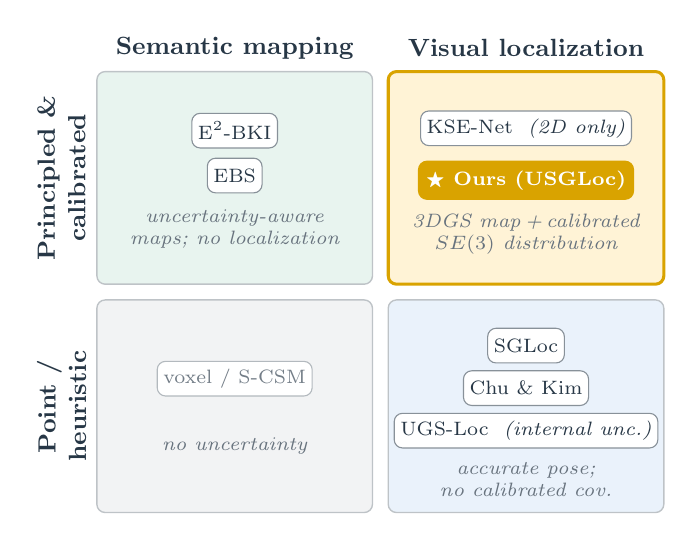
\begin{tikzpicture}[
  font=\footnotesize\color{ink},
  cell/.style={rectangle, rounded corners=3pt, draw=ink!30, line width=0.5pt,
               minimum width=3.5cm, minimum height=2.7cm},
  pill/.style={rounded corners=3pt, draw=ink!55, fill=white, line width=0.4pt,
               font=\scriptsize\color{ink}, inner sep=2.2pt, minimum height=4.4mm},
  pillf/.style={rounded corners=3pt, draw=ink!35, fill=white, line width=0.4pt,
                font=\scriptsize\color{ink!65}, inner sep=2.2pt, minimum height=4.4mm},
  pillO/.style={rounded corners=3pt, draw=outLn, fill=outLn, line width=0.5pt,
                font=\scriptsize\bfseries\color{white}, inner sep=2.6pt, minimum height=4.8mm},
  note/.style={font=\scriptsize\itshape\color{ink!70}, align=center, text width=33mm},
  hdr/.style={font=\small\bfseries\color{ink}, align=center, text width=34mm},
  rhdr/.style={font=\small\bfseries\color{ink}, align=center, rotate=90}
]

% ---- quadrant cells ----
\node[cell, fill=mapprin] (tl) at (-1.85, 1.45) {};
\node[cell, fill=ourstr, draw=outLn, line width=1.1pt] (tr) at ( 1.85, 1.45) {};
\node[cell, fill=mappt]   (bl) at (-1.85,-1.45) {};
\node[cell, fill=locpt]   (br) at ( 1.85,-1.45) {};

% ---- column / row headers ----
\node[hdr] at (-1.85, 3.10) {Semantic mapping};
\node[hdr] at ( 1.85, 3.10) {Visual localization};
\node[rhdr] at (-4.05, 1.45) {Principled \&\\calibrated};
\node[rhdr] at (-4.05,-1.45) {Point /\\heuristic};

% ---- TL: mapping + principled ----
\node[pill] at (-1.85, 2.05) {E$^2$-BKI};
\node[pill] at (-1.85, 1.48) {EBS};
\node[note] at (-1.85, 0.80) {uncertainty-aware\\maps; no localization};

% ---- BL: mapping + point ----
\node[pillf] at (-1.85,-1.10) {voxel / S-CSM};
\node[note]  at (-1.85,-1.95) {no uncertainty};

% ---- BR: localization + point/heuristic ----
\node[pill] at (1.85,-0.68) {SGLoc};
\node[pill] at (1.85,-1.22) {Chu \& Kim};
\node[pill] at (1.85,-1.76) {UGS-Loc~~{\itshape(internal unc.)}};
\node[note] at (1.85,-2.38) {accurate pose;\\no calibrated cov.};

% ---- TR: localization + principled  (Ours) ----
\node[pill]  at (1.85, 2.08) {KSE-Net~~{\itshape(2D only)}};
\node[pillO] at (1.85, 1.42) {$\bigstar$~Ours (USGLoc)};
\node[note]  at (1.85, 0.74) {3DGS map\,+\,calibrated\\$SE(3)$ distribution};

\end{tikzpicture}
\end{document}
